\documentclass[12pt]{ucsddissertation}
% mathptmx is a Times Roman look-alike (don't use the times package)
% It isn't clear if Times is required. The OGS manual lists several
% "standard fonts" but never says they need to be used.
\usepackage{mathptmx}
\usepackage[NoDate]{currvita}
\usepackage{array}
\usepackage{tabularx}
\usepackage{booktabs}
\usepackage{ragged2e}
\usepackage{microtype}
\usepackage[breaklinks=true,pdfborder={0 0 0}]{hyperref}
\usepackage{graphicx}
\usepackage{subcaption}
\usepackage{amsmath}
\usepackage{enumitem}
\usepackage{arydshln}
\AtBeginDocument{%
	\settowidth\cvlabelwidth{\cvlabelfont 0000--0000}%
}

%commands

\newcommand{\sword}{SwordBox}
\newcommand{\thesistitle}{Disaggregated Data Structures: Sharing and contention with RDMA and Programmable Networks}

\usepackage{multirow}
\usepackage{tikz}
\newcommand*\nullcirc[1][1ex]{\tikz\draw (0,0) circle (3pt);} 
\newcommand*\halfcirc[1][1ex]{%
  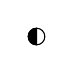
\begin{tikzpicture}
  \draw[fill] (0,0)-- (90:3pt) arc (90:270:3pt) -- cycle ;
  \draw (0,0) circle (3pt);
  \end{tikzpicture}}
\newcommand*\fullcirc[1][1ex]{\tikz\fill (0,0) circle (3pt);} 

% OGS recommends increasing the margins slightly.
\increasemargins{.1in}

% These are just for testing/examples, delete them
\usepackage{trace}
%\usepackage{showframe} % This package was just to see page margins
\usepackage[english]{babel}
\usepackage{blindtext}
\usepackage{ifthen}
\usepackage[normalem]{ulem} % for \sout
\usepackage{xcolor}
\usepackage{amssymb}

\newcommand{\ra}{$\rightarrow$}
\newboolean{showedits}
\setboolean{showedits}{true} % toggle to show or hide edits
\ifthenelse{\boolean{showedits}}
{
	\newcommand{\ugh}[1]{\textcolor{red}{\uwave{#1}}} % please rephrase
	\newcommand{\ins}[1]{\textcolor{blue}{\uline{#1}}} % please insert
	\newcommand{\del}[1]{\textcolor{red}{\sout{#1}}} % please delete
	\newcommand{\chg}[2]{\textcolor{red}{\sout{#1}}{\ra}\textcolor{blue}{\uline{#2}}} % please change
}{
	\newcommand{\ugh}[1]{#1} % please rephrase
	\newcommand{\ins}[1]{#1} % please insert
	\newcommand{\del}[1]{} % please delete
	\newcommand{\chg}[2]{#2}
}

\newboolean{showcomments}
\setboolean{showcomments}{true}
% \setboolean{showcomments}{false}
\newcommand{\id}[1]{$-$Id: scgPaper.tex 32478 2010-04-29 09:11:32Z oscar $-$}
\newcommand{\yellowbox}[1]{\fcolorbox{gray}{yellow}{\bfseries\sffamily\scriptsize#1}}
\newcommand{\triangles}[1]{{\sf\small$\blacktriangleright$\textit{#1}$\blacktriangleleft$}}
\ifthenelse{\boolean{showcomments}}
%{\newcommand{\nb}[2]{{\yellowbox{#1}\triangles{#2}}}
{\newcommand{\nbc}[3]{
 {\colorbox{#3}{\bfseries\sffamily\scriptsize\textcolor{white}{#1}}}
 {\textcolor{#3}{\sf\small$\blacktriangleright$\textit{#2}$\blacktriangleleft$}}}
 \newcommand{\version}{\emph{\scriptsize\id}}}
{\newcommand{\nbc}[3]{}
 \renewcommand{\ugh}[1]{#1} % please rephrase
 \renewcommand{\ins}[1]{#1} % please insert
 \renewcommand{\del}[1]{} % please delete
 \renewcommand{\chg}[2]{#2} % please change
 \newcommand{\version}{}}
\newcommand{\nb}[2]{\nbc{#1}{#2}{orange}}

\definecolor{ibcolor}{rgb}{0.4,0.6,0.2}
\newcommand\iv[1]{\nbc{IB}{#1}{ibcolor}}
\usepackage{wasysym}
\newcommand\yesml[1]{\nbc{ML {\textcolor{yellow}\sun}}{#1}{mircolor}}

\definecolor{sgcolor}{rgb}{0.2,0.0,0.5}
\newcommand\sg[1]{\nbc{SG}{#1}{sgcolor}}

\definecolor{samcolor}{rgb}{0.2,0.4,0.2}
\newcommand\sam[1]{\nbc{SC}{#1}{samcolor}}

\definecolor{hccolor}{rgb}{0.21,0.54,0.84}
\newcommand\hc[1]{\nbc{HC}{#1}{hccolor}}

\definecolor{ideacolor}{rgb}{1.0,0,0.5}
\newcommand\idea[1]{\nbc{IDEA}{#1}{ideacolor}}


\definecolor{abstractcolor}{rgb}{0.0,0.5,1.0}
\newcommand\rabstract[1]{\nbc{ABSTRACT}{#1}{abstractcolor}}

\definecolor{introcolor}{rgb}{0.0,1.0,0.5}
\newcommand\rintro[1]{\nbc{INTRO}{#1}{introcolor}}

\definecolor{papercolor}{rgb}{1.0,1.0,0.0}
\newcommand\rpaper[1]{\nbc{PAPER}{#1}{papercolor}}

\definecolor{multicolor}{rgb}{1.0,0,0}
\newcommand\rmulti[1]{\nbc{MULTI}{#1}{multicolor}}

% Todo Command
\definecolor{todocolor}{rgb}{0.9,0.1,0.1}
\newcommand{\todo}[1]{\nbc{TODO}{#1}{todocolor}}


\overfullrule5pt
% ---

% Required information
\title{\thesistitle}
\author{Stewart Steven Grant}
\degree{Computer Science}{Doctor of Philosopy}
% Each member of the committee should be listed as Professor Foo Bar.
% If Professor is not the correct title for one, then titles should be
% omitted entirely.
\chair{Alex C. Snoeren}
% Your committee members (other than the chairs) must be in alphabetical order
\committee{Amy Ousterhout}
\committee{Yiying Zhang}
\committee{George Papen}
\degreeyear{2024}

% Start the document
\begin{document}
% Begin with frontmatter and so forth
\frontmatter
\maketitle
\makecopyright
\makesignature
% Optional
\begin{dedication}
\setsinglespacing
\raggedright % It would be better to use \RaggedRight from ragged2e
\parindent0pt\parskip\baselineskip

\textit{To my inner circle -- Family, Loved ones and Friends. And to every belayer that caught me. Thanks for the proverbial and literal support.}


% In recognition of reading this manual before beginning to format the
% doctoral dissertation or master's thesis; for following the
% instructions written herein; for consulting with OGS Academic Affairs
% Advisers; and for not relying on other completed manuscripts, this
% manual is dedicated to all graduate students about to complete the
% doctoral dissertation or master's thesis.

% In recognition that this is my one chance to use whichever
% justification, spacing, writing style, text size, and/or textfont that
% I want to while still keeping my headings and margins consistent.
\end{dedication}
% Optional
\begin{epigraph}
\vskip0pt plus.5fil
\setsinglespacing
{\flushright

"If this is the best of possible worlds, what then are the others?"\\
\vskip\baselineskip
-Voltaire \textit{Candide}\par}

\vfil
\begin{center}

\noindent “It must be considered that there is nothing more difficult to carry out, nor more
doubtful of success, nor more dangerous to handle, than to initiate a new order of things.”

\vskip\baselineskip
\hskip0pt plus1fil -Niccolo Machiavelli \textit{The Prince}\hskip0pt plus4fil\null

\end{center}
\vfil
"If every porkchop were perfect we wouldn't have hotdogs"\\

\vskip\baselineskip
-Greg Universe, \textit{Steven Universe}

\vfil
\end{epigraph}

% Next comes the table of contents, list of figures, list of tables,
% etc. If you have code listings, you can use \listoflistings (or
% \lstlistoflistings) to have it be produced here as well. Same with
% \listofalgorithms.
\tableofcontents
\listoffigures
\listoftables

% Preface
% \begin{preface}
% \todo{Write a preface - take a look at some examples because it seems rather free form}
% Almost nothing is said in the manual about the preface. There is no
% indication about how it is to be typeset. Given that, one is forced to
% simply typeset it and hope it is accepted. It is, however, optional
% and may be omitted.
% \end{preface}

% Your fancy acks here. Keep in mind you need to ack each paper you
% use. See the examples here. In addition, each chapter ack needs to
% be repeated at the end of the relevant chapter.
\begin{acknowledgements}

I would like to acknowledged my advisor Alex C. Snoeren for his dedication to his craft and guidance
over the past 6 years. No piece of work within this thesis would be possible without your
collaboration. I would also like to thank my committee members Amy Ousterhout, Yiying Zhang, and
George Papen for their feedback and guidance, and Srikanth Kandula for his mentorship during my time
at MSR.

This thesis has been extraordinarily influenced by Anil Yelam, my closest collaborator. Thank you
for all the time you spent working on our collaborations, and the hours spent discussing and
debating system designs and performance results. I'm forever grateful. To Maxwell Bland, your
research energy is unmatched and without your help we would never have have acquired any SmartNICs.
And Alex (Enze) Liu for his superior knowledge of Python and unmatched focus on research.  Thank you
to all of the members of the Systems and Networking group at UCSD, especially the optical networking
group for your feedback and guidance during the first years of my PhD.

Thank you to Meta for funding my research and providing me with the opportunity to work on resource
disaggregation, Cavium for the generous donation of two SmartNICs, and to ARPAe for funding my first
years of research.

I'd like to thank all of the members of 3140 for their collaboration and friendship over the years.
It's truly the best office, Chez bob volunteers for keeping me fed, and to my friends for the
support. Camille Rubel thanks for having the best climbing schedule in the world, Phillip Arndt for
pushing my limits, and Camille Moore for keeping me on my toes.
\todo{double check I thanked everyone}


\end{acknowledgements}

% Stupid vita goes next
\begin{vita}
\noindent
\begin{cv}{}
\begin{cvlist}{}
\item[2012-2016] Bachelor of Science, Computer Science University of British Columbia
\item[2016-2018] Master of Science, Computer Science University of British Columbia
\item[2018-2024] Doctor of Philosophy, Computer Science University of California, San Diego
\end{cvlist}
\end{cv}

% This puts in the PUBLICATIONS header. Note that it appears inside
% the vita environment. It is optional.
\publications

\noindent Deepak Bansal and Gerald DeGrace and Rishabh Tewari and Michal Zygmunt and James Grantham
and Silvano Gai and Mario Baldi and Krishna Doddapaneni and Arun Selvarajan and Arunkumar Arumugam
and Balakrishnan Raman and Avijit Gupta and Sachin Jain and Deven Jagasia and Evan Langlais and
Pranjal Srivastava and Rishiraj Hazarika and Neeraj Motwani and Soumya Tiwari and Stewart Grant and
Ranveer Chandra and Srikanth Kandula. 2023. Disaggregating Stateful Network Functions. In
proceedings of 20th USENIX Symposium on Networked Systems Design and Implementation (NSDI 23).
Usenix Association, Boston MA, USA, 1469--1487.
https://www.usenix.org/conference/nsdi23/presentation/bansal \\

\noindent Stewart Grant, Anil Yelam, Maxwell Bland, and Alex C. Snoeren. 2020. SmartNIC Performance
Isolation with FairNIC: Programmable Networking for the Cloud. In Proceedings of the Annual
conference of the ACM Special Interest Group on Data Communication on the applications,
technologies, architectures, and protocols for computer communication (SIGCOMM '20). Association for
Computing Machinery, New York, NY, USA, 681–693. https://doi.org/10.1145/3387514.3405895 \\

\noindent Stewart Grant, Hendrik Cech, and Ivan Beschastnikh. 2018. Inferring and asserting
distributed system invariants. In Proceedings of the 40th International Conference on Software
Engineering (ICSE '18). Association for Computing Machinery, New York, NY, USA, 1149–1159.
https://doi.org/10.1145/3180155.3180199 \\


% This puts in the FIELDS OF STUDY. Also inside vita and also
% optional.
% \fieldsofstudy
% \noindent Major Field: Computer Science
\end{vita}

% Put your maximum 350 word abstract here.
\begin{dissertationabstract} 
%%	
Resource disaggregation proposes a next-generation architecture for data center resources. System
components like compute, memory, storage, and accelerators are separated from one another by a fast
network and composed dynamically into virtual servers when required. This paradigm promises
dramatically improved resource utilization, scalability, and flexibility, but introduces dramatic
challenges in terms of performance and fault tolerance. Memory is among the most difficult resources
to disaggregate. CPUs currently expect DRAM to ultra low latency, high bandwidth, and to share it's
failure domain. In particular increased latency from network round trips dramatically shifts the
performance of existing shared data structures designed for local DRAM.

In this thesis I explore the challenges of sharing disaggregated memory with hundreds of CPU cores.
First in {\sword} I present a system which utilizes a centralized programmable switch to cache data
structure state and dramatically improve key-value workload performance. Second I present a new
key-value store RCuckoo which is designed to leverage RDMA and reduce round trips when accessed by
CPU's over a network. Both systems demonstrate significant performance improvements over the
existing state of the art.

\end{dissertationabstract}

% This is where the main body of your dissertation goes!
\mainmatter

% Optional Introduction
\begin{dissertationintroduction}

\textit{What should a data center server look like?} 20 years ago a data center operator may have
argued for the simplicity of homogeneity over optimal performance, reasoning that carefully picked
hardware at a given price point would yield the best cost-performance tradeoffs and that the
performance yields of next generation hardware would quickly erase any gains made by specializing
servers. 
%%
Since then both Moors law and Dennard scaling have slowed down dramatically. CPU clock speeds and
memory density improvements have stagnated leaving operators to fight tooth and claw to enjoy the
efficiency gains of prior decades. The effect is that new technologies are being introduced to to
achieve scaling.  CPU's are now monstrously parallel. custom accelerators are common for common
workloads like video coding, and machine learning. Indeed the modern datacenter is a hodgepodge of
heterogeneous hardware (GPU's, TPU's, DPU's, SmartNICs and FPGA's)~\cite{nitro}, and various new
memory offerings and tiers like NVMe. Today the same operator that argued for homogeneity would
likely be unable to name every kind of server in their data center. At the time of writing EC2 has
84 listed instance types~\cite{ec2-offer} for their customers to design their services. The trend is
clear, in search of efficiency data center and server design is increasingly heterogeneous with
servers being designed for specific applications and workloads.

Resource disaggregation is a new architectural paradigm for data center resources aimed at improving
efficiency and managing increased heterogeneity. In the disaggregated model a servers resources do
not monolithic reside in a 1, 2, or 4U server form factor, instead each resource i.e compute,
memory, storage is dedicated to a single machine and interconnected via a fast network. Servers are
composed dynamically from these resources which enables them to be provisioned for their exact
purpose. This model enables resource pooling and sharing which in turn leads to higher efficiency.

% DRAM in particular has quickly become a precious resource in the data center. Main memory capacity,
% while growing has not kept up with CPU core counts. The result is that per-core memory capacity is
% less than 10 years ago~\cite{micron-memorywall}. New memory tiers like NVMe have been introduced to
% help alleviate memory pressure from applications, but the composition of these memory tiers, and the
% software to manage them are still undecided.

DRAM in particular has become a precious resource in data centers and is a focused target for
resource pooling~\cite{micron-memorywall}. The benefits of pooling are clear when examining a
simple bin packing problem. Consider 2 servers both provisioned with 4GB of DRAM and 3 jobs each of
which requires 2.5GB of memory. In a monolithic design a scheduler can only place one job per
machine or risk swapping to disk. In a disaggregated model the 4GB of memory would be placed in an
8GB pool which could easily subdivided into 3 2.5GB partitions. In the monolithic case the unused
memory is stranded, pooling reclaims stranded memory.  More concretely at datacenter levels
practitioners have to provision their servers for the sum of peak demand, when resources are pooled
they can be provisioned for the peak of the sum of demand which can be significantly
lower~\cite{supernic, dsnf}.

Disaggregation is only possible because of new fast and programmable networks. Commodity NICs now
offer 400Gbps with expectations for continued growth, and network devices are increasingly
programmable with multiple vendors offering programable SmartNICs, DPUs and switches.  These two
trends have lead to intra rack latencies of 1-2us and network bandwidths on the same order as memory
bandwidths with the ability to inspect, cache, and modify packets in flight at line rate.
%%
But if disaggregation were easy it would have been done already, \textit{and it some cases it has}.
Storage, has seen widespread disaggregation. The key enabling factor is that storage device access
latency is far higher than a network round trip. In the case of memory the opposite is true. Memory
access latency is 20x lower than an RTT effectively making it a separate tier of memory when placed
across a network.  This performance gap plays out in dramatic fashion when porting data structures
designed for local memory to far memory systems. Sharing data between multiple remote machines where
coherence between remote cores is required leads to abysmal performance degradation (300x tail
latencies in some cases). Further complicating the design of shared data structures is that memory,
once in a single fault domain, can fail ripping a hole directly into a processes address space.

This thesis explores the design of shared data structures in disaggregated memory systems.  I
present two systems ({\sword} and RCuckoo) which focus on the challenges of sharing and contending
access to remote memory. {\sword} (Chapter~\ref{chap:swordbox}) is a middlebox approach for removing
contention from shared data structures. The high level insight behind {\sword} is to leverage the
fact that at rack-scale TORs have a serialized view of traffic to and from servers. Using this idea
{\sword} caches data structure state on a programmable switch. 
%%
Second I present RCuckoo (Chapter~\ref{chap:rcuckoo}) a fully disaggregated key-value store. RCuckoo
is specially designed to improve key-value locality. Using locality sensitive hashing RCuckoo
improves, reads, writes, locking and fault recovery performance buy reducing the overall number of
round trips required for each operation.
%%
{\sword} yields orders of magnitude improvements in both
throughput (up to 30x) and tail latency (up to 300x).  RCuckoo meets or exceeds the performance of
all state of the art disaggregated key-value stores on small key-value pairs and significantly
outperforms other systems on read-mostly workloads.

\end{dissertationintroduction}

\chapter{Background}

Calls for distributed memory systems have been made for decades, and the groundwork of
disaggregation relies heavily on the work of the past~\cite{treadmarks,gms}. However, disaggregation
differs from prior distributed systems due to it's scale, and system assumptions. Disaggregation
assumes that each resource be stand alone, and paired with miniscule or no compute power, save for
resources like CPUs an GPUs which are inherently compute.  This assumption transforms the
technologies and requirements for disaggregated systems. Critically Remote Direct Memory Access
(RDMA) (or a similar CPU bypass technology) is essential in constructing a passive storage system.

\section{Disaggregation}

As with many paradigm shifts within the systems community the idea of disaggregation is born from
shifting hardware trends. Per core access to memory has been decreasing for decades. CPU core counts
have consistently increased for over a decade while memory speeds and capacity have improved
comparatively slowly~\cite{micron-memorywall}. The result is that CPU cores have less access to
memory now than 10 years ago. Memory is now an increasingly scarce resource and data center
operators are exploring new ways to achieve better memory utilization. Disaggregation is one such
option. Monolithic servers have a fixed amount of RAM per machine which, at a data center level,
leads to a skewed distributed of memory utilization. Some servers are starving for memory while
others have gigabytes to spare. This spare (stranded) memory is one target of disaggregation, it
aims to give each server access to a shared pool of RAM. In general a disaggregated resource, be it
memory, FPGA's, or the network itself, can be provisioned for the peak-of-sums, rather than
monolithic resources which are provisioned for the sum-of-peaks~\cite{clio,supernic,dsnf}.

The biggest barrier to disaggregation is network latency, and more aptly the difficulty of
disaggregating a resource is proportional it's access latency with respect to the additional latency
of the network. Disaggregated storage is a foregone conclusion. Academias and industry have pooled
SSD's and HDD's into shared storage pools for their increased capacity and lower cost. This is
relatively easy in comparison to an accelerator, or memory as the access cost of storage is already
high relative to the network. In concrete terms intra rack RDMA ping latencies are on the order of
1-2 us. HDD latencies are 10-20ms and SSD are often 100's of us. In these cases the network overhead
is a single digit percentage or less~\cite{decible}. In contrast DRAM latencies are 50-100ns. DRAM
over RDMA has a nearly 20x overhead compared to local access. Despite this overhead RDMA is one of
the strongest contenders for a disaggregated transport.  CXL is a burgeoning technology which
promises NUMA like latencies for remote memory access~\cite{cxl}. At the time of writing CXL is not
widely available and it's performance and scalability are not well understood. Regardless of
interconnect the principle of access latency remains the same. This thesis focuses on RDMA although
we see the algorithms and data structures presented here to be largely interconnect independent.


\section{RDMA}

Remote direct memory access (RDMA) is a low latency, high bandwidth network protocol. It achieves
high performance by bypassing multiple overheads common to a traditional networking stack (ex Linux
Sockets). Firstly RDMA is a kernel bypass technology. It allows user space applications to directly
interact with the network interface card (NIC). This removes two distinct overheads, context
switching and data copy to the kernel. Second, RDMA's most distinguishing feature is that it
offloads much of the network stack to the NIC hardware, and bypasses the CPU entirely for data
transfer. As an example, in a traditional networking stack if a process sends a UDP message on an
existing socket the user first marshals the data and then submits it to the kernel via a
\textit{send}. The kernel then copies the data out of user space, sets up the packet header, and
submits the packet to the NIC. In contrast with RDMA the user space application registers a region
of memory with the NIC prior to sending data. If an application wants to transfer the data in that
region to a remote machine it passes a pointer to the data, and the data's size to the NIC along
with the remote machines's address, and the action the NIC should take (read, write, ect). The
application sends by calling a special \textit{rdma send}. This operation is non-blocking and sends
a signal to the NIC which then DMA's the memory out of the processes address space, constructs a
packet on the NIC (including managing transport state) and sends directly to another machine. The
receiving NIC (in the case of a write), issues the DMA to the remote machine's memory without ever
interacting with it's CPU.  The example above is only a high level overview of an RDMA write, the
RDMA protocol is deeply complex. The current infiniband RDMA specification is over 1700
pages~\cite{infiniband-spec}. In this section I will briefly cover the most important aspects of
RDMA for the purposes of this thesis.

\subsection{One-Sided Verbs}

The RDMA specification provides 5 service types (Reliable Connection, Unreliable Connection,
Reliable Datagram, Unreliable Datagram, RAW Datagram). Additionally RDMA provides \textit{Verbs}
actions the NIC can take, which vary by service type. Reliable services provide acknowledgements and
connection services provide sequence numbers, in-order delivery, and retransmission. Service type
determines which verbs are available for use. Reliable connections provide the strongest guarantees
and allow for the use of \textit{one-sided} verbs which implement memory-like semantics. One sided
verbs entirely bypass the CPU of the remote machine and allow a client to directly read, write, and
atomically modify the remote hosts memory. This ability makes RDMA a powerful tool for designing
disaggregated systems, especially memory systems as it allows designers to build with the assumption
that memory is passive i.e no remote CPU exists. This prototyping ability is quintessential for
understanding how future disaggregated systems will perform.

The memory semantics of one sided RDMA are complex. Not all verbs respect ordering even on the same
connection. RDMA provides a variety of configurations to gain ordering both on and across
connections. Queue pairs (QPs) are connection handles for RDMA. Verbs are issued on a QP and QP are
polled for responses. QP's provided in-order delivery, but not necessarily in-order completion. For
instance issuing a read prior to a write may see the results of the write. Across QP no ordering is
guaranteed by default. RDMA provides two atomic operations compare and swap (CAS) and fetch and add
(FAA) for atomic modification of 64 bit regions of remote memory. The RDMA advanced transport
supports masked versions of these operations to allow for high density atomic regions while reducing
contention~\cite{rdma-masked-cas}. These atomic operations are the critical component for building
shared disaggregated systems. They enable the construction of locks and semaphores, as well as
lock-free data structures.

\section{CXL}

RDMA is not the only proposal for disaggregated memory. The Compute Express Link (CXL) is a new
interconnect and standard supported by chip manufacturers and hyperscalers. CXL is built on PCIe and
aims to expand CPU memory capacity by allowing for the attachment of remote memory devices. Despite
only a few CXL devices being available at the time of writing the technology is promising. Initial
work has shown that CXL latencies for remote memory devices are between 2-5x the latency of local
memory demonstrating that CXL devices can provide lower latency and higher throughput than
RDMA~\cite{cxl-demyst,tpp,pond}. Given these promising results we expect that CXL will be a strong
contender for remote memory pools.

CXL has limitations that are not present in RDMA, specifically surrounding how memory is shared. CXL
provides cache coherent memory semantics, however the expected cost of coherence similar to NUMA
coherence will be high. Second CLX does not currently support a routing layer which limits it to the
scalability of a CXL switch (likely rack scale). Finally CXL does not, at the time of writing,
support in-network programmability. As we will show in our work in Chapter~\ref{chap:swordbox}
in-network programmability is a powerful tool for reducing contention in shared data structures, the
lack of any programmable devices in network may limit the ability to effectively share CXL devices.
Prior work on remote memory data structures indicated that allowing CPU cores to subscribe to
\textit{notify} groups could reduce the price of coherence while enabling fast shared
structures~\cite{aguilera2019designing}. While notifications are not natively supported by CXL, CXL
devices could be designed to support them without the need to build CXL programmable network
devices. 

Alternatively techniques for NUMA scalability may also apply to remote such as black box approaches
for NUMA data structures~\cite{bbn,nros,ironsync}. These techniques are powerful and enable general
data structures to be built on NUMA architectures with low latency. While powerful these systems
require each NUMA domain to synchronize it's log with a singular log master, it also requires
efficient support for atomic operations like CAS. It's unclear at this point in time if these
approaches will scale up to the expected number of NUMA domains in a disaggregated deployment due to
the fact that their bandwidth requirements grow linearly with the number of domains.

\section{Programable Networks}

The past decade has seen the rise of programmable network devices. These devices are capable of
executing users code often at line rate. A huge variety of devices exist: SmartNICs~\cite{fairnic},
DPUs, FPGAs, and programmable switches~\cite{p4} from a wide variety of vendors. Often these devices
provide thin operating systems which allow users to develop and deploy code, either C or P4. These
programmable devices are powerful and transformational tools for designing network systems as they
can offer orders of magnitude performance improvements when deployed in the right
context~\cite{when-computer}, such as sequencing where it has show to offer huge benefits for
consensus~\cite{eris, nopaxos}. In this thesis we leverage the power of programmable switches to
exactly this benefit to get fast in-network serialization for RDMA based data structures (Section
~\ref{chap:swordbox}).

Programmable switches differ from other programmable network devices in that they have orders of
magnitude more aggregate bandwidth, specific pipeline architecture, and exclusively operate on P4
programs.
%%
Programmable switches such as Intel Tofino~\cite{tofino2} utilize a pipeline architecture. Switches
typically have an ingress and egress pipeline which is broken into multiple stages. In the case of
Tofino 2 both ingress and egress have 12 stages. Packets pass through one or more stages and are set
for transmission once each stage of the pipeline used by the program has executed. Per stage
computation is limited, usually to a few instructions, such a fetching from a lookup table
processing a conditional, or modifying and storing packet header data. The result is that P4
programs have a constrained programming model. Loops and recursion are not easily supported and
branching is limited. Finally switch memory is highly constrained per pipeline stage. All P4
accessible memory is SRAM of which each switch only has a few megabytes.
%%
Ideal programs for programmable switches provide a high degree of benefit from a small amount of
computation. As an example a network sequencer which gives a unique monotonic sequence number to
each packet is ideal as it requires only a few small amount of storage space, and limited amount of
computation per packet.

\subsection{Programmable Switch Use (and Misuse) Cases}

Memory constraints on programmable network devices, as well as their programming model and
architecture have a large impact on what kinds of systems can and should be built upon
them~\cite{when-computer}. Cache size and pipeline depth have a large impact on what can be
effectively stored on a programable switch. As part of our exploration of {\sword}
(Chapter~\ref{chap:swordbox}) we examined the use of a programmable switch as a cache for the
replicated log, and found that the switch for a variety of subtle reasons was not a good fit for our
cache despite many prior works on in-network caching and key-value
stores~\cite{netcache,netchain,netkv,netlock}.

In the log system all clients must read all log entries for consistency. This read patten leads to a
bandwidth bottleneck on the server hosting the log as the number of clients increases and the size
of the log entry increases.  Figure~\ref{fig:bandwidth-model} Illustrates how as the number of
clients and the size of individual log entries increases performance falls over. In our initial
design we debated how to deal with the bottleneck. On one hand we could replicate the log across
multiple memory servers and alleviate the broadcast bottleneck by spreading it across replicas.
Alternatively we could cache the most recent writes on a programmable switch.  Initially we thought
that the switch would be an excellent place for the log cache because we could easily reason about
the access pattern of the log, and each client's link bandwidth would be proportional to how much
they read. But the devil is in the details. Due to RDMA and switch pipeline constraints as described
in the following section we found that the switch was an untenable solution.

\begin{figure}
\centering
\includegraphics[width=0.99\linewidth]{fig/bandwidth-model.pdf}
\caption{Bandwidth model for memory replication. 1MS is a single memory node, while 3MS is 3.}
\label{fig:bandwidth-model}
\end{figure}

\begin{figure}
    \centering
    \includegraphics[width=0.5\textwidth]{fig/switch-cache-model.pdf}
    \caption{Performance improvement of caching on a programable switch as a function of hit rate and object cache size}
    \label{fig:switch-cache-model}
\end{figure}

The values in Figure~\ref{fig:switch-cache-model} assume 64 clients and a single memory server and a
log entry size of 8 bytes. The 0\% hit rate on cache sizes of 1024 is almost identical to the
furthest left point in Figure~\ref{fig:bandwidth-model} with 64 clients and a single memory node.
Note that with this cache size and a hit rate of 95\% which may be attainable considering the log
access patterns are extremely predictable we are able to handle around 200 Million ops per second.

Unfortunately current programmable switch hardware does not allow for cashable objects over 192
bytes. Our Tofino 2 switch has a fixed sized 64 bit maximum storage capacity at each stage of it's
pipeline, with a total of 24 stages counting both ingress and egress~\cite{tofino2}. Given a maximum
cache size of 192 we can again calculate our maximum performance improvement. Using max sized RDMA
reads of 192 bytes we significantly drop performance without the use of a switch, and in the common
case get around 68 MOPS, our model without a switch striping across 3 memory servers yields a
maximum of 57 MOPS. While still a theoretical advantage we consider the complexity of adding a
programmable switch and caching for and 18\% benefits to be not worth it, especially considering
that next generation NICs are slated for bandwidths of 800GBPS+. If future switch technology were to
allow for larger object caches we believe this direction may be fruitful.

Given these kinds of subtle constraints the use of programmable network hardware must be carefully
considered. In the case of \sword we explore the use of a programmable switch for caching parts of a
shared data structure including locks, and parts of index structures. We found that some data
structures, specifically those that require very little state in their index for a read or a write
to succeed are well suited for caching. An example of this is appending to a linked list where only
the last element of the list needs to be cached in order for an append to succeed. Alternatively
inserting into an arbitrary location in a linked list is hard as all the nodes in the linked list
need to be cached.

\section{Disaggregated Systems and Data Structures}

The trends and technologies discussed in the above sections have lead to a new class of system for
disaggregation. These systems are built with the assumption that resources are separated by a fast
network and have little to no heterogeneity. I.e a storage server will be prominently storage which
minimal compute to boot and configure the machine and execute simple management
tasks~\cite{aguilera2019designing,fast-networks,dis-and-app,legoos}.

Disaggregated memory is the focus of many systems. A common model for disaggregated memory is the
same as GMS with the exception that memory is passive and not part of a workstation pool~\cite{gms},
that is remote memory can be used as a swap space or as a remote cache rather than disk. In this
model applications are apportioned a partition of remote memory for it's
pages~\cite{infiniswap,fastswap,leap,blade-server,legoos,hydra}, objects~\cite{aifm,carbink}, or
cache lines~\cite{kona}. These systems focus on improving performance by reducing the number of
remote memory accesses that an application has to make. In general this is done by identifying hot
and cold memory then prefetching and evicting data to reduce the number of faults to remote memory.
Additionally these systems focus on fault-tolerance by replicating or erasure coding memory across
replicated memory servers~\cite{hydra}.

A commonality between each of these memory systems is the lack of sharing. Operations common to
non-disaggregated systems like mmapping a shared page are not supported by these systems. In cases
where shared access is supported using POSIX interfaces performance is not considered to be a
concern~\cite{Regions}. Disaggregated systems that share efficiently, at the time of writing, are
entirely custom built data structures, the majority of which are key-value stores, transaction
processors or caches~\cite{clover, sherman, race, fusee, rolex, ford, ditto}. Each of these system
takes on a significant burden in terms of development. Most develop their own fault tolerance,
replication, recovering, allocation, and serialization protocols. In nearly every case the
performance of these systems is determined by the techniques used to serialize writes on the index
of the data structure.
%%
The techniques used by these systems is largely the same as those used to design RDMA key-value
stores for non-disaggregated memory over the past decade~\cite{pilaf,cell,herd,farm}. The primary
difference is that disaggregated systems use exclusively one sided RDMA operations, while RDMA
key-value stores typically route write operations through a CPU to serialize requests.
%%
A few systems have proposed to or realized the potential of using a programmable switch, or NIC in a
disaggregated rack to aid in serialization. Notably MIND~\cite{mind} implements memory management on
a switch, while Clio~\cite{clio} and SuperNIC~\cite{supernic} use an FPGA based smartNIC to
implement any number of memory side network functions.





\chapter{Swordbox: Accelerated Sharing of Disaggregated Memory}
\label{chap:swordbox}

\section{Overview}

Proposals for disaggregated memory systems often forgo sharing entirely in favor of partitioned
regions~\cite{infiniswap,fastswap,leap,legoos,blade}. Each of these proposals cuts at a fundamental
goal of remote memory which is to increase capacity via pooling and reduce the need to increase CPU
pin counts for increased memory bandwidth. The unfortunate result is that these systems do not meet
the same expectations as local memory systems. For instance any system requiring mmap with
\textit{Shared} semantics is not natively supported, and for those that do, the performance penalty
is extreme with no tools to mitigate the cost. The issue with this approach is that it may have
unforeseen consequences in terms of memory utilization that may actually be worse than those on
monolithic servers. 

One strategy to deal with the cost of synchronization is to simply have applications duplicate
resources rather than share them. On a large system hosting hundred of VM's the cost of duplicating
shared libraries is known to be high and dedup among VM's is already common.  Further on monolithic
servers the explicit nature of message passing systems has been studied extensively and extremely
high performance can be achieved by using explicit remote accesses~\cite{herd, erpc}. Given these
two factors monolithic servers with well designed RPC systems could potentially share more
effectively and achieve better resource utilization than a naive disaggregated system which exposes
a transparent but slow interface to remote memory or which blindly replicates rather than sharing.

The key motivation behind {\sword} is to provide an upper bound on the performance achievable by a
disaggregated shared memory. We noticed while investigating shared remote memory that the fastest
RDMA key-value stores used mostly one-sided RDMA but still required a CPU to serialize writes. The
moment that the CPU was removed entirely the 99th percentile tail latency jumped
dramatically~\cite{clover}. One option we considered was to use a smartNIC to serialize writes
rather than a CPU, prior projects like Clio~\cite{clio}, SuperNIC~\cite{supernic}, and
Prism~\cite{prism} suggested that network functions were a good fit for smartNICs and that they
could be used to implement \textit{close to memory} operations like pointer chasing. While we
agreed, individual NICs could not provide rack-scale coherence -- in order to provide a rack-scale
uniform memory machine we would need to think about a centralized solution. A programmable switch is
an ideal candidate for this role as it sees all of the traffic in a rack and can enforce global
ordering. Our goal in this project was to design a system which could provide a full upper bound on
the performance achievable by a disaggregated shared memory system as a benchmark for future systems
to compare to.


\input{swordbox/intro}
\input{swordbox/backv2}
\input{swordbox/tmp_sigcomm}
\input{swordbox/implementation}
\input{swordbox/eval}
\input{swordbox/limitations}
\input{swordbox/conclusion}


\chapter{Disaggregated Cuckoo Hashing}
\label{chap:rcuckoo}
\section{Overview}

While \sword provides an upper bound on the performance of a shared remote memory system, it is not
a general purpose solution. While \sword is able to provide faster locking and faster optimistic
concurrency it does not handel all data structure, and more importantly, requires the addition of a
programable switch to the network. The need for programmable hardware is a significant barrier to
entry for many data center operators, and while we believe that for the most performance stringent
applications the cost is worth it, we also believe that alternative solutions may be better for
average operators given their current deployments. Part of our exploration during \sword was to
investigate data structures which would be a good fit for middlebox interposition, during this
research we also explored data structures and techniques which were amenable to disaggregation in
general.


\begin{table}[h]
	%\begin{table}[h]
		\centering
		\begin{tabular}{ c | c | c | c | c | c | c | c | c }
			& project & \shortstack{read \\ inflation} & \shortstack{relaxed  \\ layout} & \shortstack{pre-\\compute} & \shortstack{OC*} & \shortstack{metadata \\ caching} & \shortstack{CC*} & \shortstack{self \\ verifing}  \\ \hline
																	%N          %R          %P          %O          %M          %C          %W          %S
	\multirow{3}{*}{\rotatebox[origin=c]{90}{\shortstack{Multicore \\ NUMA}}} & \shortstack{Flat \\ Combining}~\cite{flat-combining}   & \nullcirc & \nullcirc & \nullcirc & \nullcirc & \nullcirc & \fullcirc & \nullcirc \\ \cdashline{2-9}
			 & \shortstack{Hopscotch \\ Hash}~\cite{hopscotch}         & \fullcirc & \nullcirc & \nullcirc & \nullcirc & \nullcirc & \nullcirc & \nullcirc \\ \cdashline{2-9}
	%\multirow{1}{*}{\rotatebox[origin=c]{0}{\shortstack{NUMA}}} & \shortstack{Blackbox \\ NUMA}~\cite{black-box-numa}     &  &  &  &  &  &  &  &  \\ \hline \hline %\cline{2-10} \cline{2-10}
			& \shortstack{Blackbox \\ NUMA}~\cite{bbn}     & \halfcirc & \nullcirc & \nullcirc & \fullcirc & \fullcirc & \fullcirc & \nullcirc \\ \hline %\cline{2-10} \cline{2-10}
	\multirow{4}{*}{\rotatebox[origin=c]{90}{\shortstack{RDMA \\ Key-Value}}} & pilaf~\cite{pilaf}                                      & \nullcirc & \nullcirc & \nullcirc & \nullcirc & \nullcirc & \nullcirc & \fullcirc \\ \cdashline{2-9}
			 & farm~\cite{farm}                                        & \fullcirc & \nullcirc & \nullcirc & \fullcirc & \fullcirc & \fullcirc  & \nullcirc \\ \cdashline{2-9}
			 & herd~\cite{herd}                                        & \nullcirc & \nullcirc & \nullcirc & \nullcirc & \nullcirc & \nullcirc  & \nullcirc \\ \cdashline{2-9}
			 & cell~\cite{cell}                                        & \nullcirc & \nullcirc & \nullcirc & \halfcirc & \fullcirc & \nullcirc  & \fullcirc \\ \hline \hline
			 % & % fasst~\cite{faast}                                      & \nullcirc & \nullcirc & \nullcirc & \nullcirc & \nullcirc %& \nullcirc & \nullcirc \\ \hdashline
			 % & % erpc~\cite{erpc}                                        & \nullcirc & \nullcirc & \nullcirc & \nullcirc & \nullcirc & \nullcirc & \nullcirc \\ \hdashline
			 %& storm~\cite{storm}                                      &  &  &  &  &  &  &  \\ \cdashline{2-9}
			 % & 1RMA~\cite{1rma}                                        &  &  &  &  &  &  &  \\ \hline \hline
	%\multirow{4}{*}{\rotatebox[origin=c]{90}{\shortstack{\small Disaggregated \\ \small Datastructures }}}        & Clover~\cite{clover}                                    & \nullcirc &  \halfcirc &  \nullcirc & \fullcirc & \fullcirc  & \nullcirc & \nullcirc \\ \cdashline{2-9}
	\multirow{4}{*}{\rotatebox[origin=c]{90}{\shortstack{\small Disaggregated \\ \small Datastructures }}}        & Clover~\cite{clover}                                    & \nullcirc &  \halfcirc &  \nullcirc & \fullcirc & \fullcirc  & \nullcirc & \nullcirc \\ \cdashline{2-9}
	%\multirow{5}{*}{\rotatebox[origin=c]{90}{\shortstack{Far-Memory \\ Structures}}}        & Clover~\cite{clover}                                    & \nullcirc &  \halfcirc &  \nullcirc & \fullcirc & \fullcirc  & \nullcirc & \nullcirc \\ \cdashline{2-9}
			 & \shortstack{RACE}~\cite{race}            & \fullcirc  & \fullcirc & \halfcirc & \fullcirc & \fullcirc & \nullcirc & \fullcirc \\ \cdashline{2-9}
			 & \shortstack{Sherman \\ ~\cite{sherman}}                            & \fullcirc & \fullcirc & \halfcirc & \fullcirc & \fullcirc & \fullcirc & \fullcirc \\ \cdashline{2-9}
			 %& Ford~\todo{}                                          &  &  &  &  &  & \\ \cdashline{2-9}
			 & Mind~\cite{mind}                                              & \nullcirc & \halfcirc & \halfcirc & \nullcirc & \fullcirc & \nullcirc & \nullcirc \\ \hline
		\end{tabular}
	
		\caption{Cross section of systems and techniques. Full circles
		\fullcirc imply that a system uses the category, \halfcirc denotes when a
		system meets the qualification in spirit but not explicitly, and \nullcirc
		when the technique is absent. Columns OC and CC stand for Optimistic Concurrency and Compute Coalescing respectively.}
		
		\label{tab:re-table}
	\end{table} 

Table~\ref{tab:re-table} is the result of a literature review on the state of the art for shared
data structures. Our reading lead us to the insight that multi-core NUMA systems and RDMA key-value
stores shared the most with new breeds of disaggregated data structures. NUMA systems had a focus on
high latency memory and techniques on how to mitigate their cost, and RDMA key-value stores
explored both techniques for high performance RDMA and how to reduce the need for serialization down
to a few fast operations~\cite{cuckoo-improvements}.

A number of threads stood out to us during our review. Perhaps the most important is that data
locality can dramatically improve performance~\cite{farm}. One of the biggest performance killers
are the additional round trips required to resolve indirect pointers. A common design pattern in
key-value stores is to have a index with a pointer to the data, and potentially long chains where
collisions occur~\cite{race, clover}. Each time a pointer resolution is required the client must
incur an additional round trip. In NUMA literature (and even for spinning disks) locality was
identified as an important factor for performance~\cite{bbn,hopscotch}. Techniques like hop-scotch
hashing ensure that data is close to it's hash location in physical memory. This is advantageous for
RDMA systems as a single big read can guess at the location of the data and be ensured to grab it
only incurring an additional bandwidth penalty.

The second trend we identified is that pushing computation to the client can save a significant
amount of time in place of locality. Page tables are difficult to port to remote memory as each
level of indirection requires a round trip. Clio introduced the idea of a flat page table. Their
insight is that when creating a virtual address space the virtual address itself is not critical.
Rather than handle multiple levels of page tables they push the complexity to the allocation
function. When allocating in Clio the allocator uses a flat hash based page table with a single look
up. The table avoids collisions by iteratively generating virtual addresses until one is produced
which does not cause a hash table collision. This \textit{pre-computation} technique is powerful as
it allows for a single round trip for getting remote memory allocations.

Table~\ref{tab:re-table} lists multiple other techniques which cross cut the literature. We believed
that techniques such as precomputation and locality could be used to improve the performance of
existing data structures. We designed our next system RCuckoo with the intuition that cuckoo
hashing, which had already been studied in the context of RDMA key-value stores, could be improved
and made highly efficient by applying these techniques.


\input{rcuckoo/intro}
\input{rcuckoo/background}
\input{rcuckoo/body}
%\input{problems}
\input{rcuckoo/design}
\input{rcuckoo/evaluation}
%\input{limitation}
\input{rcuckoo/conclusion}

% \chapter{Black Box Disaggregation}

% \section{Overview}
% \todo{finish up you writeup for a fall submission of BBD and paste it her}

\chapter{Conclusion}

This thesis proposes two systems for sharing remote memory. {\sword}, a programmable switch based
caching system which removes contention from existing disaggregated programs, and RCuckoo a cuckoo
hash designed specifically for one-sided RDMA access. Both systems push the performance and
scalability limits of shared disaggregated data structures at two points in the design space (with
and without programmable network devices). \sword demonstrates how caching can be used to remove
contention entirely and achieve performance equal to the underlying network capabilities. RCuckoo
demonstrates that by carefully constructing algorithms we can increase locality and take advantage
of features in commodity network hardware (large sequential RDMA reads, and on-NIC lock tables).

These two systems only demonstrate two design points where many more could exist. For instance,
\sword takes the stance that a single programable switch sees all traffic within the rack and
that a developer has unfettered access P4 to which programs run on the switch. Similar strategies
could potentially be used with a less generic programming interface such as openflow, as
demonstrated by netkv~\cite{netkv} however the data structures may require serious redesign to adapt
to openflows limited programming model.

Many off the shelf ARM based or FPGA based smartNICs could be used to implement \sword as well as
more complex data structures. While SmartNICs lack a global view of a rack, ARM based smartNICs do
have a global view of the machine they are attached to and could be used to implement similar
caching strategies. SmartNICs typically have much more available memory than programmable switches
and could likely handel much larger data structures than \sword. The example used at multiple points
throughout this work for a \textit{difficult} data structure for \sword to deal with is insert into
a linked list (because the entire linked list needs to be stored in memory). This is unlikely to be
the same on a smartNIC with a few GB of memory. SmartNICs could be used to cache index structures
for large structures like B-Tress and use their limited compute to steer read and write requests
similar to \sword. More generically they could be used for some of the simple functions which are
difficult to implement in remote memory such as an allocator, or scheduler which needs to maintain
centralized state.

A further and more generic option for NIC designers is to extend the interface for RDMA to better
accommodate complex one-sided data structures, while calls for pointer chasing are common, calls for
more complex atomic operations are less present~\cite{prism,clio}. The algorithms community has
designed many wait-free and lockless data structures such as binary trees, and heaps, and other
simple structures which make use of multi-cas, the ability to CAS multiple addresses simultaneously
could open up disaggregation to many pointer based data structures which would currently be
unimplementable. Simultaneously CAS and FAA are limited width.  Extensions for larger CAS sizes
would enable more efficient data structures such as in the case of RACE, and FUSEE which must limit
the size of its key-value pairs due to the lack of space in the 64 bit RDMA CAS.

Network-datastructure codesign is a powerful, but under explored area. In the case of \sword Clover
was a good fit for the system as only the tail pointer of linked lists needed to be stored on the
switch. Other data structures do not always exhibit this property. Log based or append only data
structures have promise here as the point of contention (the end of the log) can be managed with
relatively little state. Future work could be done to enable \textit{append-mostly} data structures,
Sherman for instance enjoys a degrees of associativity at its leaf nodes by having associative
leaves. Other data structures may be able to take advantage of similar properties like appending
updates to a shared log and eventually combining them into a consolidated data structure.

\sg{Most proposals for disaggregated systems are focused on rack scale deployments, as intra rack
latencies get lower and lower, and disaggregated technology gets better intra-rack solutions will
become more tennable. An early example is \textit{Disaggregating Stateful Network
Functions}~\cite{dsnf} and \textit{SuperNIC}\cite{supernic} which take the stance that a large pool
of dedicated accelerators can provide a significant portion of the network functions for a data
center. In line of work routing is paramount and under-explored. \sword assumes a centralized model
as it needs to track an entire data structure, however a future distributed model could potentially
scale to multiple racks if the data dependent operations were routed through the correct network
components.}


% \chapter{ Example Figures and such for formatting reference}
% This demonstrates how OGS wants figures and tables formatted. For
% figures, the caption goes below the figure and ``Figure'' is in bold.
% See Figure~\ref{fig:zen}. Tables are formatted with the caption above
% the table. See Table~\ref{tab:bad}.

% Of course, Table~\ref{tab:bad} looks horrible. It should probably be
% formatted like Table~\ref{tab:good} instead.

% For facing caption pages, see Table~\ref{tab:facing}. Of course,
% facing caption pages are vaguely ridiculous and my implementation of
% them in the class file is by far the most brittle part of the
% implementation. It's entirely possible that something has changed and
% these don't work at all. I implemented it merely for the challenge.

% \begin{figure}
% \centering
% \fbox{\parbox{.9\linewidth}{%
% 	\noindent
% 	{\Huge PHD ZEN}\par
% 	\vskip.5in
% 	\centerline{comic here}
% 	\vskip.5in
% }}
% \caption[``Ph.D. Zen'']{Comic entitled ``Ph.D. Zen'' by Jorge Cham, 2005. Copyright
% has not been obtained and so it isn't displayed.}
% \label{fig:zen}
% \end{figure}

% \begin{table}
% \centering
% \caption[Electronic Dissertation Submission Rates]{Electronic
% Dissertation Submission Rates at UCSD, Fall 2005 and Winter 2006.
% (First two quarters that the program was available to all Ph.D.
% candidates not in a Joint Doctoral Program with SDSU.)}
% \label{tab:bad}
% \begin{tabular}{|*{5}{>{\centering\arraybackslash}m{.15\linewidth}|}}
% \hline
% &Ph.D.s awarded (Including Joint degrees) & Electronic submission of
% Dissertation & Paper Submission of Dissertation & Percentage of
% Electronic Submission\\
% \hline
% Fall\par 2005 & 84 & 37 & 47 & 44.05\%\\
% \hline
% Winter\par 2006 & 64 & 42 & 22 & 65.63\%\\
% \hline
% \end{tabular}
% \end{table}

% \begin{table}
% \centering
% \caption[Electronic Dissertation Submission Rates]{Electronic
% Dissertation Submission Rates at UCSD, Fall 2005 and Winter 2006.
% (First two quarters that the program was available to all Ph.D.
% candidates not in a Joint Doctoral Program with SDSU.)}
% \label{tab:good}
% \renewcommand\tabularxcolumn[1]{>{\RaggedRight\arraybackslash}p{#1}}
% \begin{tabularx}{.9\linewidth}{lcccc}
% \toprule
% &\multicolumn{1}{X}{Ph.D.s awarded (Including Joint degrees)}
% &\multicolumn{1}{X}{Electronic submission of Dissertation}
% &\multicolumn{1}{X}{Paper Submission of Dissertation}
% &\multicolumn{1}{X}{Percentage of Electronic Submission}\\
% \midrule
% Fall 2005 & 84 & 37 & 47 & 44.05\%\\
% Winter 2006 & 64 & 42 & 22 & 65.63\%\\
% \bottomrule
% \end{tabularx}
% \end{table}

% \begin{facingcaption}{table}
% \caption[UCSD Gender Distribution]{University of
% California, San Diego Gender Distribution for the Campus Population,
% October~2005\\
% (http://assp.ucsd.edu/analytical/Campus\%20Population.shtml)\\
% \emph{(This is an example of a facing caption page, the next page is
% the example of the table/figure/etc.\ that corresponds to this
% caption. It is also an example of table/figure that is rotated 90
% degrees to fit the page.)}}
% \label{tab:facing}
% \renewcommand\tabularxcolumn[1]{>{\RaggedLeft\arraybackslash}p{#1}}
% \parindent=0pt
% \setbox0=\vbox{%
% \vsize\textwidth
% \hsize\textheight
% \linewidth\hsize
% \columnwidth\hsize
% \textwidth\hsize
% \textheight\vsize
% \begin{tabularx}{\linewidth}{lXXXXXX}
% \toprule
% & \multicolumn{2}{c}{\textbf{Women}}
% & \multicolumn{2}{c}{\textbf{Men}}
% & \multicolumn{2}{c}{\textbf{Total}}\\
% \cmidrule(l){2-3}\cmidrule(l){4-5}\cmidrule(l){6-7}
% \textbf{Population Segment}
% & \multicolumn{1}{c}{\textbf{N}} & \multicolumn{1}{c}{\textbf{\%}}
% & \multicolumn{1}{c}{\textbf{N}} & \multicolumn{1}{c}{\textbf{\%}}
% & \multicolumn{1}{c}{\textbf{N}} & \multicolumn{1}{c}{\textbf{\%}}\\
% \midrule
% Students & 12,987 & 51\% & 12,686 & 49\% & 25,673 & 100\%\\
% Employees & 9,943 & 56\% &  7,671 & 44\% & 17,614 & 100\%\\
% \addlinespace
% \hfill\textbf{Total} & \textbf{22,930} & \textbf{53\%} &
% \textbf{20,357} & \textbf{47\%} & \textbf{43,287} & \textbf{100\%}\\
% \bottomrule
% \end{tabularx}
% \singlespacing

% \emph{Notes}:
% \begin{enumerate}
% \item The counts shown below will differ from the official quarterly
% Registrar's registration report because 1) data for residents in the
% Schools of Medicine and Pharmacy and Pharmaceutical Science are
% excluded, and 2) registered, non-matriculated, visiting students are
% included.
% \item Student workers are excluded from employees; however emeritus
% faculty and others on recall status are included.
% \end{enumerate}

% Campus Planning. Analytical Studies and Space Planning\\
% 31 January 2006
% }
% \centerline{\rotatebox{90}{\box0}}
% \end{facingcaption}

% % This will give us some more text
% % \Blinddocument

% % Skipping a bunch of chapters
% \begin{figure}
% \centering
% \fbox{\hbox to.8\linewidth{\hss Another figure\hss}}
% \caption{Another figure caption}
% \end{figure}
% \begin{table}
% \centering
% \caption{Another table caption}
% \begin{tabular}{ccc}
% \toprule
% X&Y&Z\\
% \midrule
% a&b&c\\
% \bottomrule
% \end{tabular}
% \end{table}
% \begin{figure}
% \caption{ASDF fig}
% \end{figure}
% \begin{table}
% \caption{ASDF tab}
% \end{table}

\appendix
% \Blinddocument
\bibliographystyle{plain} % Or whatever style you want like plainnat

\bibliography{thesis}

% Stuff at the end of the dissertation goes in the back matter
\backmatter

\end{document}
